%================================================
\chapter{Kernel-Based Social Strength Modeling} \label{sec:ssm-framework}
%================================================

In this chapter, we apply kernel learning techniques to address the challenging problem of Social Strength Modeling (SSM) of users in a social media community. In particular, we take Flickr---the most popular online photo sharing community---as an example, in which users are sharing their experiences through substantial amounts of multimodal contents (e.g., photos, tags, geo-locations, friend lists) and social behaviors (e.g., commenting and joining interest groups). Such heterogeneous data in Flickr bring opportunities yet challenges to research community for SSM. One of the key issues in SSM  is how to effectively explore the heterogeneous data and how to optimally combine them to measure the social strength. In this chapter, we present a kernel-based learning to rank framework for inferring the social strength of Flickr users. In the first stage, we employ kernel target alignment algorithm to integrate heterogeneous data into a holistic similarity space. With the learned kernel, in the second stage, we rectify the pair-wise learning to rank framework to estimate the social strength among Flickr users. By learning the social strength graph, we are able to conduct collaborative recommendation and collective classification on a large-scale data set crawled from Flickr. The promising results show that the learning-based approach is effective for SSM. Although focused on Flickr, our technique could be naturally applied to model social strength of users in other social media community, such as Facebook, Twitter, and so on.

%================================================
\section{Problem Setting}\label{sec:ssm-formulation}
%================================================

Social network mining (SNM), from communication networks, to friendship networks, to professional and organizational networks,
has attracted a surge of interests in both industrial and academic communities. Most traditional studies focus on detecting {\em
binary} relation ties between people (e.g., friends or not). Such a coarse indicator is not precise enough to give insight about the strength of
social relationship among people. Some recent work, e.g., the study in \cite{www/XiangNR10}, has attempted to address the problem of {modeling the strength of
social connections} instead of simple binary linkage prediction. Inferring precise social strength can facilitate a variety of applications, including
friendship linkage prediction, item recommendation, social search, and so on.

\begin{figure*}[!t]
\includegraphics[width=\linewidth]{figures/mm_framework.eps}
%\vspace{-3cm}
\caption{Illustration of our kernel based learning to rank framework. The first panel shows the data of three users, based on which we have three graphs in the
second panel (we omit other possible graphs for illustration purpose). In the third panel, we first learn the weight $\bm\theta$ by maximally aligning the
combination to the friend graph. Then we adopt learning to rank framework with logistic loss to estimate the social strength.}
\end{figure*}

In this chapter, we investigate the challenging problem of Social Strength Modeling (SSM) of users in social media communities. In particular, we adopt Flickr,
the most popular and largest online photo sharing portal, as the social media platform in our study. Flickr contains rich user-generated contents, including
sharing photos, user-annotated tags, comments, etc. Analogues to other social networking sites, e.g., {\em Facebook} and {\em LinkedIn}, each Flickr user can
add other users into contact list to indicate their friendship. Users can also create and join interest groups where users share photos of common interests.
Besides the explicit mutual linkage relationship between users, the uploaded photos and their associated metadata (tags, comments, etc.) can also be leveraged to infer the similarity and implicit relationship between users. The versatile information available on Flickr poses a unique opportunity yet challenges for the research on SSM.

One key challenge of SSM is to effectively explore and combine heterogeneous data from multiple modalities to measure the social strength in a principled
manner. Previous work on Flickr data mining has predominately focused on image-only or tag-only analysis. The other rich metadata has not been well exploited. To overcome the limitation of existing work, we present a novel framework for social strength modeling by unifying multi-modal heterogeneous data through a kernel-based machine learning approach. In particular, we suggest to use {\it kernel machine}~\cite{ml/CortesV95} to compute user similarity between users in each modality of Flickr data, and further propose a two-stage learning scheme to measure social strength by kernel-based learning techniques.

Specifically, we assume the final proximity graph of users is a linear combination of multiple proximity graphs derived from all the modalities in Flickr. Each proximity graph is computed by defining a kernel function on each modality. At the first learning stage, we propose to combine the multiple proximity graphs by learning the optimal combination by following the kernel target alignment principle in kernel learning theory~\cite{icml/CortesMR10,nips/CristianiniSEK01}. At
the second learning stage, we propose a kernel-based learning to rank the social strength of users with the optimal kernel learned from the previous stage. The
proposed two-stage learning approach is able to model the social strength of users by exploring multi-modal heterogeneous contents in social media communities in a systematic and comprehensive way. It is worth noticing that although we take Flickr as a particular example of social media community (as Flickr opens a public way to access its rich metadata, which are more comprehensive and formal than other social sites), the proposed learning approach can be applied to any kind of community such as Facebook and LinkedIn, in which users are also associated with multi-modal metadata.

By learning the continuous social strength between users, our technique can facilitate a number of real-world social media applications. In particular, we apply our technique to devise interest item recommendation and collective classification social tasks. To summarize, this chapter makes the following major
contributions:
\begin{itemize}
\item We study the problem of modeling social network strength of users in a social media community. To the best of our knowledge, this is the first work focused on this particular topic in multimedia research community.
\item We propose a novel two-stage kernel-based learning framework for social strength modeling, which effectively integrates heterogeneous data by optimally combining multiple kernels, and learns to rank social strength of users by a kernel-based learning to rank approach.
\item We conduct extensive experiments to evaluate the performance of our technique on a large-scale real-world dataset, and found encouraging insights and knowledge about social connections in social multimedia platform like Flickr.
\end{itemize}

The rest of the section is organized as follows. Section \ref{sec:ssm-formulation} formulates the problem of social strength modeling on Flickr data. Section \ref{sec:ssm-framework} presents the proposed framework. Section \ref{sec:ssm-experiment} discusses our experiments. Section \ref{sec:ssm-discussion} reviews related works.

\begin{figure*}[!t]
%\hspace{-1.5cm}
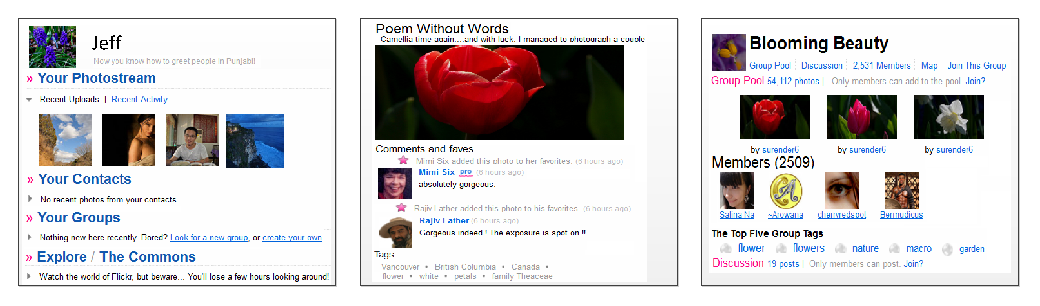
\includegraphics[width=\linewidth]{figures/mm_sample.eps}
%\vspace{-1cm}
\caption{Illustration of the elements (both photos and the rich metadata) of a typical Flickr user (Left), a Flickr image (Middle), and Flickr interest group
(Right). }
\end{figure*}

In this section, we give the problem definition of social strength modeling. We commence by summarizing the list of frequently used symbols in Table 1. For math notations used in this chapter, we use upper case letter to denote a variable, curlycue upper case letter to denote a space, and bold case letter denote a matrix or a vector.

\begin{table}[h]
\label{table:notation}
\begin{center}
\caption{List of frequently used symbols.}
\begin{tabular}{|c|l|}
\hline
Symbol & Description\\
\hline
\hline
$\N_u$ &$\{1,\ldots,u\}$, a set of integers up to $u$\\
$N_u$ &$|\N_u|$, the cardinality of $\N_u$\\
%$p$ & a Flickr photo\\

$u_i$ & the $i$-th Flickr user\\
%$\hat{u}_i$ &$[u_{i1}, u_{i2}]$ an ordered pair of Flickr users\\
$\U$ &$\{\u_i: i\in\N_u\}$, a collection of $N_u$ users\\
%$g$ &a Flickr interest group\\
$X,T,D,L,\mathcal C$ & attributes of a Flickr photo: picture, tags, \\
&date, location, and comments, respectively\\
$\mathcal P, \G, \mathcal N$ & a collection of Flickr photos, groups, \\
&and friends, respectively\\
$\#$ &the number of some object\\
$K,\K$ &a similarity / kernel function and matrix\\
\hline
\end{tabular}
\end{center}
\end{table}

First of all, we formally define the problem of social strength modeling with Flickr data below.

\begin{definition}[Social Strength Modeling]
Given a collection of Flickr users $\U$, the goal of a {\em social strength modeling} problem is to learn a function $f:\U\times\U\rightarrow \mathbb{R}_+$ such
that $f(\u_i, \u_j)$ measures the strength of social relationship between user $\u_i$ and user $\u_j$.
\end{definition}
In the above definition, a basic element is a Flickr user $\u_i\in\U$, which can be defined below. %object we deal with is Flickr user $U$, which is abstracted
to be
\begin{definition}[Flickr user]
Each {\em Flickr user} $\u_i\in\U$ is modeled as a three-dimensional tuple $\u_i:=[\mathcal P, \mathcal N, \mathcal G]$, where $\mathcal P = \{p_i:i\in\N_z\}$
is a collection of Flickr photos uploaded by user $\u_i$, $\mathcal N \subset \U$ is the collection of users who appear in the contact list of user $\u_i$,
$\mathcal G$ is the collection of interest groups joined by user $\u_i$.
\end{definition}
In the above definition, $\mathcal N$ and $\mathcal G$ indicate the explicit social relationship and organizations of Flickr users, and $\mathcal P$ may be
beneficial to disclosing some implicit relationship between users. We discuss each of them below. The left picture in Figure 2 is an intuitive example of Flickr
user. {\em Your Photostream, Your Contacts,} and {\em Your Groups} correspond to $\mathcal P$, $\mathcal N$, and $\mathcal G$, respectively.

The contact list $\mathcal N$ indicates the binary social ties between users. Note that the friend relationship given by $\mathcal N$ is often asymmetric, which can be naturally handled by our proposed learning to rank framework in the next section. We employ $\mathcal N$ as the training data of known social strength for building our model.


The set $\mathcal G$ is the interest groups the user $\u_i$ has joined. For each $g\in\mathcal G$, it is created and self-organized by registered Flickr users.
Users belonging to the same group tend to share photos of common interests. The right picture in Figure 2 show a popular interest group.

The photos $\mathcal P$ are useful to find implicit social relationship since they contain rich context information that expresses user interest and the
communication between users. We formally define a Flickr photo below.
\begin{definition}[Flickr image]
A {\em Flickr photo} is defined as 5-dimensional tuple $P:=[X, T, D, L, \C]$, where
\begin{itemize}
  \item $X\in\mathcal X\subset\R^{d_x}$ is a visual picture under some fixed-length feature representation, $d_x$ is the dimension of images;
  \item $T\in\mathcal T\subset\R^{d_t}$ is a vector representing the tags associated with $X$, $d_t$ is the size of tag vocabulary;
  \item $D$ is the date that $X$ is created;
  \item $L:=[latitude, longitude]\in\R_+\times\R_+$ is the location where $P$ is created;
  \item $\C:=\{[U, C]_i \in \mathcal U \times \R^{d_t}:i\in\N_c\}$ is a collection of comments of $P$, where the first component $U$ is the user who posts
the comment and the second component $C$ is the content of the comment.
\end{itemize}
\end{definition}

The rich context information ($T, D, L, \C$) besides the uploaded photo $X$ encode social communication information between users. The middle picture shows an example of Flickr users. In this chapter, we incorporate them into a unified discriminative framework to model the social strength.

%================================================
\section{Kernel-based Social Strength Modeling} \label{sec:ssm-framework}
%================================================

In this section, we propose a kernel-based learning framework for social strength modeling.

%++++++++++++++++++++++++++++++++++
\subsection{Motivations}
%++++++++++++++++++++++++++++++++++

Referring to Figure 2 which illustrates the data we are dealing with here. The first challenge is how to combine such heterogeneous data effectively. Note that we can compute the similarity $K$ under different modality, which is akin to a kernel function in kernel machines including support vector machine and kernelized logistic
regression. This inspires us the multiple kernel learning (MKL) scheme to integrate the multiple modalities, which has been actively studied in recent years
since the pioneering work \cite{jmlr/LanckrietCBGJ03}. Though not always yielding better results than single kernel chosen by cross-validation\cite{icml/Cortes09}, it is indeed
useful in combining heterogeneous data sources (e.g., in bioinformatics\cite{bmcbi/YuFDTSMM10}). Therefore, we make use of the-state-of-the-art MKL algorithm \cite{icml/CortesMR10} to weight each modality.

Second, we notice the social strength essentially ranks the degree of affinity between a pair of people. Therefore, we adopt the pair-wise learning to rank framework to further rectify the social strength based on the learned $K$ in the first stage. Comparing with generative models, such a discriminative model often enjoys better generalization ability \cite{Vapnik98}. Moreover, it avoids latent variable assumption and parametric-form assumption of generative model functions, which makes
the learning more compact and precise.

We first discuss how to measure similarity of Flickr users by defining a variety of kernel functions $\{K\}$ on different modalities of Flickr data. We then present a kernel learning technique to determine the optimal combination of multiple kernels following the {\em kernel target alignment} (KTA)
principle~\cite{icml/CortesMR10,nips/CristianiniSEK01}. Finally, based on the learned kernel, we formulate the social strength modeling problem into a pair-wise
kernel-based learning to rank task, which can be efficiently solved in an iterative manner as IVM~\cite{nips/ZhuH01}.

%++++++++++++++++++++++++++++++++++
\subsection{Kernels for Measuring User Similarity} \label{sec:ssm-kernel}
%++++++++++++++++++++++++++++++++++

For machine learning algorithms, the kernel trick is an important technique for mapping observations from a general set into a much higher- and possibly
infinite-dimensional inner product space without ever having to compute the mapping explicitly. Typically, every kernel $k:\mathcal S\times \mathcal S\rightarrow \mathbb{R}$ on a
set $S$ essentially defines the way of measuring similarity between data instances in the set $\mathcal S$. In this section, we present a series of candidate kernel
functions in different modalities for measuring similarity of Flickr users, which will be further explored with other kernel methods for inferring social
strength.

%--------------------------------------------------
\subsubsection{Similarity in Visual Space}
%--------------------------------------------------

For visual feature representation, we adopt the bag-of-(visual) word model. Specifically, we first extract the SIFT descriptors \cite{jcv/LoweG04}. All these
descriptors are split into $d_x$ groups by the k-Mean clustering process. Given a photo, we assign each of its SIFT descriptors to a nearest cluster center.
Then each image is converted into a fixed length vector $\x\in\R^{d_x}$, where $d_x$ is the size of visual dictionary. The $i$-th component of this vector
counts the frequency of SIFT features assigned to cluster $i$.
We measure image similarity on $\X$ by a Gaussian kernel:
\[
s(\x_i,\x_j) = e^{-\|\x_i - \x_j\|^2/\sigma^2}.
\]
where $\sigma$ is a kernel parameter. For a specific user, we employ the centroid of its images to represent its visual contents, i.e.,
\[
\bar{\u}=\sum_{\x_i\in\u} \x_i / |\u|,
\]
where $|\u |$ is the number of photos belonging to user $\u$. Thus, the similarity between two users can be measured by:
\[
K^1(\u_i,\u_j) := e^{-\| \bar{\u_i} - \bar{\u_j} \|^2 / \sigma^2}.
\]
It is difficult to obtain an optimal bandwidth parameter $\sigma$. We set it to be the average Euclidean distance empirically.

%--------------------------------------------------
\subsubsection{Similarity in Textual Space}
%--------------------------------------------------

Note each uploaded photo can be annotated with a set of possible tags by users. We adopt the bag-of-word model to represent the textual
information\cite{Baeza-YatesR99}. In particular, we collect all the tags and build a tag dictionary of size $d_t$. All the tags of an entity is converted into a
fixed length vector in $\R^{d_t}$ by the traditional {\em tf-idf} weighing method. Here the inverse document frequency is the number of users containing that
tag. We employ the normalized linear kernel which is widely used for text classification:
\[
K^2(\u_i, \u_j) := \frac{\x_i^\top\x_j}{\sqrt{\x_i^\top\x_i}\sqrt{\x_j^\top\x_j}}
\]
Comparing with the visual kernel $K^1$, the tag-based kernel carries more semantic information.

%--------------------------------------------------
\subsubsection{Similarity by Mutual Comments}
%--------------------------------------------------

The interaction between users reflects the social connection between each other. For example, if two users often post comments on each other's photos, probably they have
strong social ties. In general, people who are friends in real life would communicate more frequently. We can collect the mutual comment information between users to construct an symmetric link graph, in which each vertex represents a user and the edge weight is the number of comments between two users. Thus we have
\[
K^3(\u_i, \u_j)  = \#\mbox{Comments between } \u_i \mbox{ and } \u_j.
\]
When $i=j$, the kernel value is how many times $\u_i$ has ever posted to itself.

%--------------------------------------------------
\subsubsection{Similarity by Common Interest Groups}
%--------------------------------------------------

The Flickr users can create or join in {\em Flickr interest groups}, which consists of a collection of users who share common interest or taste on photos of specific styles. Such interest groups can help users to find people or photos of their interest. Researchers have proposed techniques (eg.,
\cite{mm/NegoescuG08,mm/NegoescuAPVG09}) to analyze the structure and themes of the groups due to their importance in organizing Flickr users. Intuitively, people among which strong social connections exist are more likely to join the same interest groups as they may affect each other and share similar interest. Therefore, we can use the number of common interest groups to measure the similarity between people:
\[
K_u^4(\u_i, \u_j) = \#\mbox{Groups both } \u_i \mbox{ and } \u_j \mbox{ joined}.
\]
When $i = j$, the kernel value is the number of groups $u_i$ has joined.

%--------------------------------------------------
\subsubsection{Similarity by Common Friends}
%--------------------------------------------------

Each Flickr user has a contact list, which can be deemed as ``friends". When two users share many common friends, it is reasonable to infer that they have strong
social connection to each other. Naturally, we can count this number as the kernel value to quantify this modality:
\[
K^5(\u_i, \u_j) =  \#\mbox{Friends belong to both }\u_i \mbox{and} \u_j.
\]

%--------------------------------------------------
\subsubsection{Similarity via Geo-tags}
%--------------------------------------------------

The social photos are often associated with geo-tags, which states the latitude and longitude where the photos are created. If two users have been traveled to
the same place frequently, it is reasonable to conclude they are similar to each other. Similar to the representation in textual space, we use the bag of
geo-tag to compute the similarity between users.
\begin{eqnarray}
K^6(\u_i, \u_j) &=& \#\mbox{Locations where both } \u_i \mbox{ and } \u_j \nonumber\\
&& \mbox{taken photos}. \nonumber
\end{eqnarray}
At the diagonal position of $K^6$, the value is the number of places the user has been to. The raw geo-tags are in form of longitude and latitude pairs. We
discrete it by dividing the whole globe into grids. Each location is represented by the lattice it belongs to.

%--------------------------------------------------
\subsubsection{Similarity via Favorite Photos}
%--------------------------------------------------

One important function provided by Flickr is that users can mark their favorite photos (fave). Assuming the number of faves correlates to the social strength,
we define
\[
K^7(\u_i, \u_j) = \#\mbox{Photos both }\u_i \mbox{ and }\u_j \mbox{ favriate}.
\]
The rationale underlying this assumption is that users who like the same photos tend to be friend. Apparently, this may not be true in real case. Through the
KTA algorithm we learn the weights of these kernels, which provides us insight about which modalities are indeed informative for detecting social strength in multimedia communities.

The similarity measures $K_u^{1\sim7}$ are not necessarily positive semi-definite (p.s.d.). We can force these measures to be p.s.d. to construct kernels by adding a properly scaled identity matrix to the corresponding similarity matrix.

%++++++++++++++++++++++++++++++++++
\section{Optimal Combination of Multiple Kernels} \label{sec:kta}
%++++++++++++++++++++++++++++++++++

In the above, we define various kernel functions for similarity measures in different modalities. The next challenge is to find the best way of combining these
modalities, which plays a key role in social strength modeling. Specially, our goal is to determine a linear combination of multiple kernels in fusing all
modalities for similarity measure:
\begin{equation}
K(\u_i, \u_j;\bm\theta) = \sum_{t = 1}^{N_k} \theta_tK^t(\u_i, \u_j), \label{eqn:multi-kernel}
\end{equation}
where $K^t$ is the kernel defined under the $t$-th view of the users, $N_k$ is the total number of views.

One naive way is to manually fix weights of different modalities, which however highly relies on domain knowledge and cannot find the optimal combination due to
the heuristic manner.
In this section, we present a kernel-based learning technique to find the optimal combination of multiple kernels by following the principle of kernel target
alignment~\cite{nips/CristianiniSEK01}.

Specially, given the target labels $\Y$, we can adopt the {\em kernel alignment}~\cite{nips/CristianiniSEK01} to measure the quality of kernel $\K$ with respect
to the target label matrix $\Y$. The formal definition of kernel alignment is defined below:
\begin{definition}[Kernel Alignment]
Let $\K\in\R^{N_u\times N_u}$ and $\Y\in\R^{N_u\times N_u}$ be two kernel matrices such that $\|\K\|_F\neq 0$ and $\|\Y\|_f\neq 0$. Then, the {\em alignment}
between $\K$ and $\Y$ is defined by
\[
\rho(\K, \Y) = \frac{\E\big[\tr\K\Y\big]}{\sqrt{\E\big[\tr\K\K\big]\E\big[\tr\Y\Y\big]}},
\]
\end{definition}
Here the expectation is taken over samples on which the kernel is evaluated.
Note that the kernel matrices usually have to be centered~\cite{icml/CortesMR10}, i.e., $\E[K_{ij}]=0$. This centering step can be simply computed from
\[
[\K]_{ij} := K_{ij}-\frac{1}{N_u}\sum_{i=1}^{N_u}K_{ij} - \frac{1}{N_u}\sum_{j=1}^mK_{ij}+\frac{1}{N_u^2}\sum_{i,j=1}^{N_u}K_{ij}.
\]
Given the target graph represented by matrix $\Y$, we maximize the alignment $\rho$ over $\K$ to solve the kernel. The matrix $\Y$ is observed from the Flickr
platform. For example, in a friend prediction task, $\Y$ is the mutual contact graph constructed from the profile of each Flickr users. Suppose we have $N_k$
modalities $\K^1,\ldots,\K^{N_k}$. We assume the target kernel is in form of $\K = \sum_{t=1}^{N_k}\theta_t\K^t$, where $0\leq \theta_t\leq 1, \sum_t\| \theta_t
\|_2= 1$. Thus the target variable is reduced from $\R^{N_u\times N_u}$ to $\mathcal M:=\big\{\|\bm\theta\|_2 = 1\wedge\bm\mu\geq 0\big\}$. The following
theorem guarantees the optimal solution can be computed immediately\cite{icml/CortesMR10}:
\begin{theorem}
The solution $\bm\theta^*$ of the optimization problem
\[
\max_{\bm\theta\in\mathcal M}\rho(\K,\Y)\;:\;\K=\sum_{t=1}^{N_k}\theta_t\K^t
\]
is given by $\bm\theta^*=\bm\theta^*/\|\bm\theta^*\|$, where $\bm\theta^*$ is the solution of the following quadratic program:
\[
\bm\theta^*=\argmin_{\bm\theta\geq \0}\bm\theta^\top\mathbf M\bm\theta-2\bm\theta^\top\mathbf a,
\]
where $\mathbf a$ is the vector $(\langle \K^1,\Y\rangle_F,\ldots,\langle \K^{N_k},\Y\rangle_F)^\top$ and $\mathbf M$ is the matrix $M_{kl}:=\langle
\K^k,\K^l\rangle_F$, for $k,l\in[1,N_k]$.
\end{theorem}

%++++++++++++++++++++++++++++++++++
\section{Kernel-based Learning to Rank}
%++++++++++++++++++++++++++++++++++

\subsection{Framework}

Let $z$ be a $\{0, 1\}$-valued latent variable to indicate whether there is a connection between two users. The social connection strength inference is about to
estimate the probability $P(z_{ij}=1|\u_i, \u_j)$. To this purpose, we build a logistic normal model based on training pairs. The connection between Flickr
users come from the mutual contact $\mathcal N$ in Flickr user profile, i.e., $z_{ij}=1 $ if and only if $\u_j$ is in the contact list of $\u_i$.

\begin{eqnarray}
\min_{\w} \frac{C}{2}\| \w \|_2^2 + \sum_{\u_i, \u_j \in \mathcal U}l(y_{ij}, \w^\top(\Phi(\u_i) - \Phi(\u_j))), \label{eqn:primal-obj}
\end{eqnarray}
where we use a linear model $f(\u_i, \u_j) = \w^\top(\Phi(\u_i) - \Phi(\u_j))$ parameterized by $\w$ to predict the social strength between $\u_i$ and $\u_j$.

The label $y_{ij} = 1 - z_{ij}$ takes value in $\{0, 1\}$ indicating the connection between $\u_i$ and $\u_j$. When $\u_i$ has $\u_j$ as a friend, we set
$y_{ij}= 0$. The function $\Phi(\cdot):\U\rightarrow\R^d$ maps a user $U$ to a feature representation under some specific view. The function $l(\cdot,
\cdot):\R\times\R\rightarrow\R_+$ measures the loss of prediction. We adopt the logistic loss $l(y_1, y_1) = \ln(1 + e^{-y_1y_2})$ instead of hinge loss in
traditional SVM-based ranking model, as it can predict the probability of classification result. Thus we can estimate the social strength by
 \[
P(z=1|\u_i, \u_j) = e^{f(\u_i, \u_j)} / (1 + e^{f(\u_i, \u_j)}).
 \]


According to the representor theorem\cite{colt/ScholkopfHS01}, the solution of the above problem can be expressed in form of $f(\hat{u}_i) =
\sum_j\alpha_jK(\hat{u}_i,\hat{u}_j)$, where $\hat{u}_i:= [\u_{i1}, \u_{i2}]$ is an ordered pair of users, $f(\hat{u}_i)$ predicts the scoring indicating the
strength between this pair of users. Thus the dual objective can be written as
\begin{eqnarray}
%\min_{\ba\in\R^{N_u}} -\y^\top(\K\ba) + \1^\top\ln(1 + \exp(\K\ba)) + \frac{C}{2}\ba^\top\K\ba, \label{eqn:dual-obj}
\min_{\ba\in\R^{N_u}} \frac{1}{N_p}\1^\top\ln\big(\1 + e^{-\y\circ(\K\ba)}\big) + \frac{C}{2}\ba^\top\K\ba, \label{eqn:dual-obj}
\end{eqnarray}
where $\K\in\mathbb S^{N_u^2\times N_u^2}$ is the kernel matrix, evaluated from a kernel function $K:(\U\times\U)\times(\U\times\U)\rightarrow\R$ defined on the
user pairs.


The kernel of two pairs $\hat{u}_i$ and $\hat{u}_j$ is computed as
\begin{eqnarray}
K(\hat{u}_i, \hat{u}_j) &=& (\Phi(\u_{i1}) - \Phi(\u_{i2}))^\top(\Phi(\u_{j1}) - \Phi(\u_{j2})) \nonumber\\
&=& K_u(\u_{i1}, \u_{j1}) + K_u(\u_{i2}, \u_{j2}) \nonumber\\
&& - K_u(\u_{i1}, \u_{j2}) - K_u(\u_{i2}, \u_{j1}) \nonumber.
\end{eqnarray}
The dual objective (3) can be solved efficiently as an im-
port vector machine (IVM)\cite{nips/ZhuH01}.

%--------------------------------------------------
\subsection{Training Pair Selection}
%--------------------------------------------------

When a user $u_j$ appears in the contact list of $u_i$, it is likely that $u_j$ is a friend of $u_i$ in real life or that the content uploaded by $u_j$ is of
the interest of $u_i$. Therefore, we can treat $(u_i, u_j)$ as a positive pair directly when training the model. However, it is not so trivial for the case of
negative pairs. It is a common case that $u_i$ has not noticed his friend $u_j$ has registered. Thus $u_i$ does not add $u_j$ into his contact list. If we
simply treat $(u_i, u_j)$ as negative training pairs, the learned model would fail to predict such latent friends effectively. Actually one of our important
applications is to reveal such potential friends. It calls for elaborate strategies for sampling negative pairs.

Moreover, there are computational necessity for training pair sampling. Suppose each user has $N_k$ friends on average, we would have $O(N_k\times(N_u -
N_k)\times N_u)$ training pairs over all. Such a large scale makes it prohibitive to apply learning to rank algorithm directly. On the other hand,
some of the training pairs are not helpful for learning the models. We propose a two-stage scheme for sampling pairs.

First, we choose the pairs of users that are least likely to be friends to construct negative training pairs. To this end, for each user $u_i$, we sort the
values $K^t(u_i, u_j)$, $1\leq t \leq N_k$ in descending order. The users with small similarity to $u_i$ are excluded from the potential friend list of $u_i$.
Since we have multiple $N_k$ kernels defined on users, it is unclear to adopt which one for the sampling purpose. Here we employ a very conservative scheme,
that is, we choose the top $N_e$ users that appear in the top $N$ ($N>N_e$) users of $u_i$ under all the similarity measures $K^t$. For constructing positive pairs, we use $K^3$, i.e., the kernel counting the mutual comments, to determine the most frequently communicate with $u_i$ as positive pairs.

Second, we adopt the active sample selection scheme in IVM \cite{nips/ZhuH01} during the training phase. Due to the logistic loss function of (\ref{eqn:primal-obj}), the solution is non-sparse. However, many of the samples are not necessary to yield a useful solution. We can actively select a pair to expand the set of support vectors at each iteration. In this way, the learning can be significantly sped up while the efficacy of the learned classifier is preserved \cite{nips/ZhuH01}.

%++++++++++++++++++++++++++++++++++
\subsection{Applications}
%++++++++++++++++++++++++++++++++++

The proposed social strength modeling framework can benefit a variety of applications, including not limited to:

{\bf Friendship Prediction.} In Flickr each user can add other registered users into his/her contact list. However, when users are known to each other in real
life, or they share quite similar interest in photo styles, the friendship link may not exist explicitly due to the limited searching and browsing
functionality. Our framework can predict the implicit links between Flickr users by leveraging the various content and context information.

{\bf Collaborative Recommendation.} It is very useful to improve user experience by recommending proper objects to users. For example, the interest groups and
favorite photos. Such item recommendation tasks can be benefited from the modeled strength as the popularity of these terms are correlated with the social
strength among people. Affinity propagation algorithms can be designed based on the learned social strength graph.

{\bf User-Targeted Advertising.} Similar to the case of object recommendation, we can provide user-targeted advertising to a connected component consisting of
similar users, so that the advertisements are relevant to user interest through a propagation among similar users.% \cite{Mei:PIEEE10}.

{\bf User Search \& Browse.} We can rank the user search results according to their social strengths with the one who conducted the query. The user is more
likely to find out the targets of his interest. This technique can compensate the lack of informative words matching with the query. Therefore, we expect the
results based on traditional simple keyword matching can be greatly improved.

{\bf Community Visualization.} The applications of visualizing people's local social network could be improved by scaling/shading links according to the
estimated relationship strengths.

%================================================
\section{Experiments} \label{sec:ssm-experiment}
%================================================

In this section, we evaluated the proposed social strength modeling techniques on a real data set crawled from Flickr. We start from a random user as seed and
expand the crawling according to its friend list in a bread first search manner. We stopped at 4,919 users as we consider such a scale is enough to work with to
conduct reliable conclusions. Besides the photos, all the associated metadata, including the ones defined in Section 2, are downloaded in XML format. We
evaluate the effect of social strength modeling on recommendation tasks.

\begin{table}[!tb]
\label{table:dataset}
\caption{The statistics about our crawled Flick dataset.}
\begin{center}
\begin{tabular}{|c|c|c|c|c|}
\hline
\#user    &\#group &\#image &\#tag &\#contact\\
\hline
\hline
4,919   &109,205    &5,001,601  &116,372 &81,447\\
\hline
\end{tabular}
\end{center}
\vspace{-3mm}
\end{table}

%++++++++++++++++++++++++++++++++++
\subsection{Friend Recommendation}
%++++++++++++++++++++++++++++++++++

\begin{figure*}[!ht]
%\hspace{-0.7in}%\centering
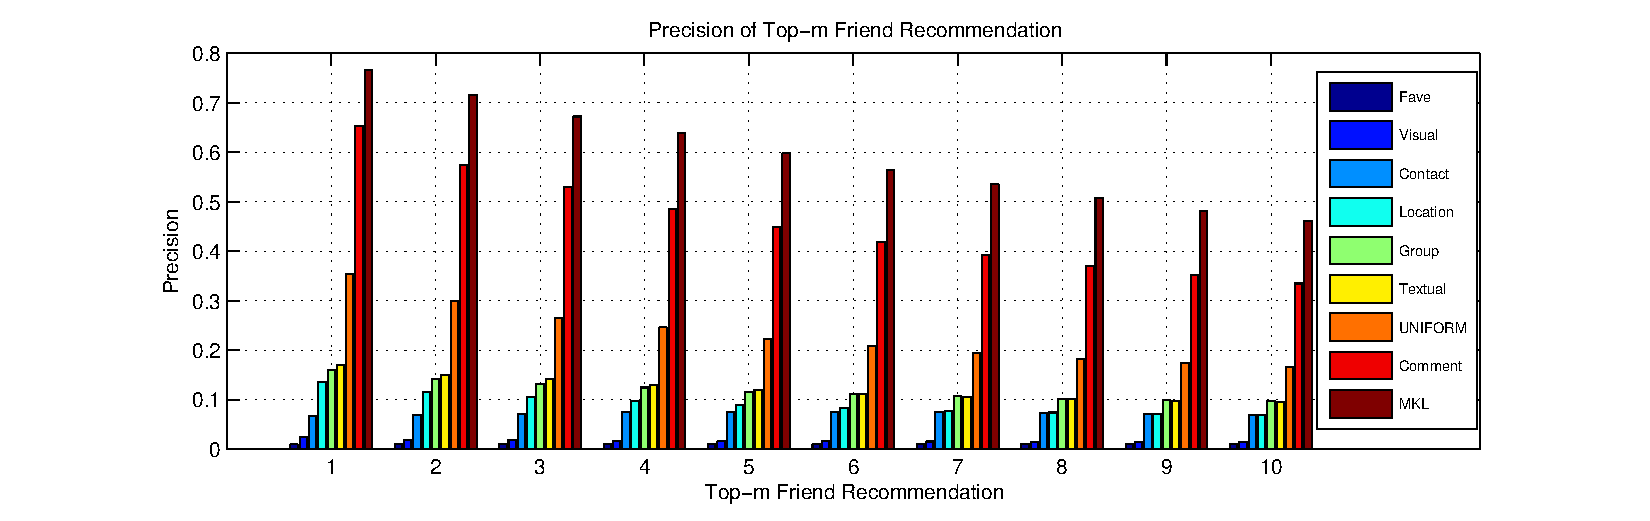
\includegraphics[width=\linewidth]{figures/friend.eps}
\caption{The average top-10 friend recommendation accuracy of single kernel and combined multiple kernels.}
\end{figure*}

\begin{table*}[t]
\centering
\caption{The base kernels and the weights by KTA in the friend and group recommendation task.}
\begin{tabular}{|c|r|r|r|r|r|r|r|}
\hline
Kernel  &1 &2 &3 &4 &5 &6 &7\\
\hline
Name &Visual &Textual &Comment &Group &Contact &Location &Fave\\
\hline
\hline
Friend &.0042   &.1007  &.6488  &.0637  &.1042  &.0499  &.0285\\
Group &.0183    &.1687  &.5065  &N/A    &.2030  &.0397  &.0299\\
\hline
\end{tabular}
\end{table*}

The essence of SSM is to infer the acquaintance between two people. Therefore, the most direct criterion of SSL is to measure the friend recommendation
accuracy. It is also an important application for social network sites (including Flickr, though it is not initially designed for social purpose).

We randomly choose 4,000 users for training purpose. The target kernel matrix $\Y$ in Section \label{sec:kta} is the friend indicating matrix. The $i$-th row of
$\Y$ is a binary vector indicating whether a user is in the contact list of user $\u_i$. We adopt the learning to rank to infer the social strength based on
kernels. For each kernel matrix $\K$, we normalize it by dividing each row with the maximal value at that row. Then we use $\K = (\K + \K^\top) / 2$ to make it
symmetric. For the ones not satisfying the positive semi-definite (p.s.d.) property (this can be examined by eigen-decomposition), we add $\delta\I$ to make
them p.s.d. The valuated kernels include:
\begin{itemize}
  \item {\em Single}: A single kernel defined in Section \ref{sec:ssm-kernel}. By examining the kernel one-by-one, one can observe the effect of each modality
clearly;
  \item {\em Uniform}: Each kernel is assigned the same kernel weight. This is the baseline showing the result of simple combination, which serves as
baseline method;
  \item {\em KTA}: The kernel target alignment method introduced in Section \ref{sec:kta}.
\end{itemize}
Given a test user, we sort the values in descending order and extract the top users as recommended friends. The learned weights of the kernels are presented in Table 3. The self-explanatory name of kernel implies its definition in Section \ref{sec:ssm-kernel}. The top-10 friend recommendation results are plotted in Figure 3. We draw several observations from the results.

First, KTA-MKLR yields the best performance among all the evaluated kernels. Its top-1 accuracy approaches 80\%, and top-10 accuracy approaches 50\%. Such relatively high accuracy confirms that inferring social strength on multimedia site is possible. It could open a new perspective for social network mining. For $m$ from 1 to 10, KTA-MKLR significantly outperforms other kernels. Specially, the naive unform combination only reports half of the accuracy of  MKL. This fact
verifies the efficacy of the proposed method. Moreover, it implies that the underlying single kernels are complementary. It coincides with previously conclusion
that MKL is effective at concatenating heterogeneous data.

Second, The {\em Comment} kernel ($K^3$) reports the second best result. Recall the definition of $K^3$, it's the number of mutual comments among Flickr users.
Its good results show that the {\em mutual communication} is still the most informative modality when inferring social strength. This fact is consistent with
the large volume of works on social network analysis, most of which are mutual communication based. Moreover, note that $K^3$ is also better than uniform
combination. It means some of the modality is actually noisy. Therefore, learning the modality weight in a principle manner is crucial. Careless combination can
actually hurt performance.

Third, we can analyze the contribution of each modality from the results of every single kernel. Specifically:
\begin{itemize}
  \item The {\em Textual} kernel ($K^2$) reports the second best accuracy among all the single kernels, though it's significantly worse than $K^3$. Thus we
can conclude that the photos of friends exhibit stronger semantically similarity. However,
  \item The {\em Visual} kernel ($K^1$) reports very poor performance. This could be possibly explained by the semantic gap. Besides, we use the mean of
photos to measure visual similarity due to the difficulty of dealing with large scale photos. This also could lose much information;
  \item The {\em Fave} kernel ($K^7$) produces the worst performance among the 7 base kernels. With $m$ varying from 1 to 10, its accuracy is most zero
consistently. This fact means it is not useful when inferring social strength;
  \item The {\em Group} kernel ($K^4$) is quite similar to {\em Textual} kernel. Their performance can be explained in the same manner as the group
membership indicate the semantics of users' photos;
  \item The {\em Location} kernel ($K^6$) is helpful as friends have higher probability residing or taking pictures at the same place.
\end{itemize}

%++++++++++++++++++++++++++++++++++
\subsection{Group Recommendation}
%++++++++++++++++++++++++++++++++++

\begin{figure*}[!ht]
%\hspace{-0.7in}%\centering
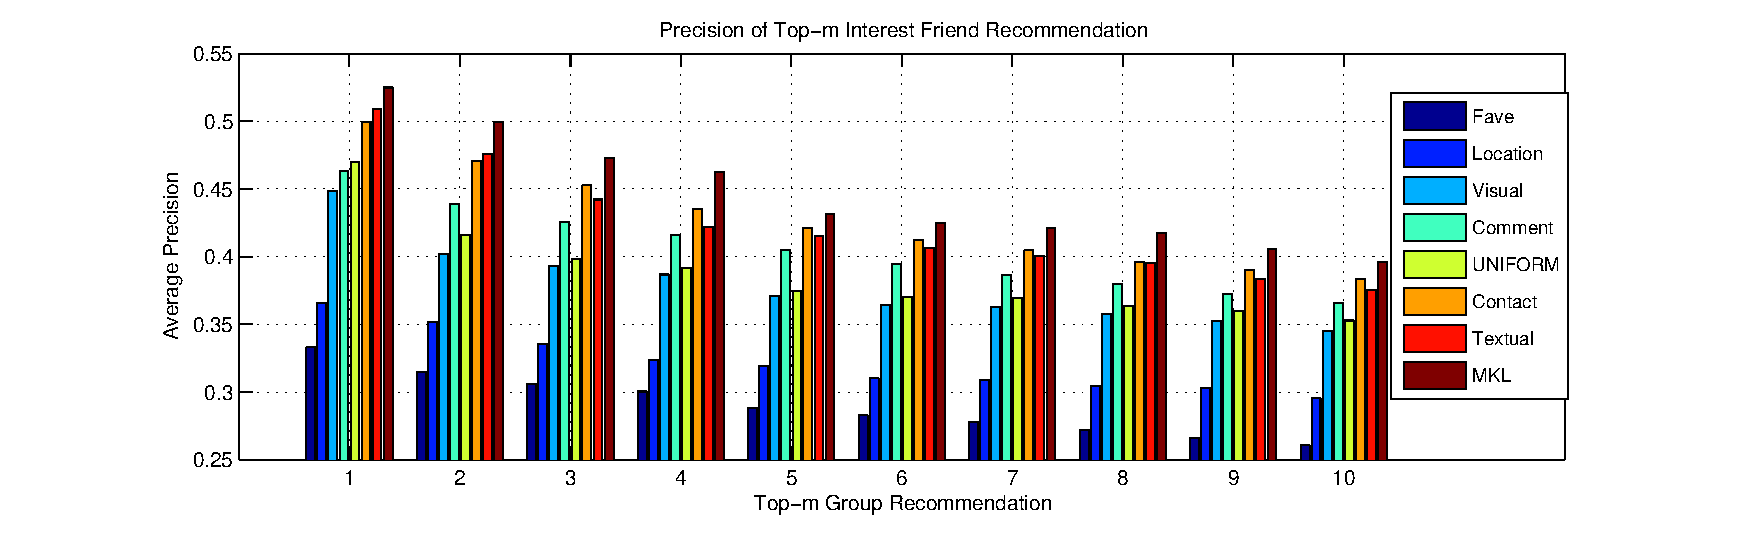
\includegraphics[width=\linewidth]{figures/group.eps}
\caption{The average top-10 group recommendation accuracy of single kernel and combined multiple kernels.}
\end{figure*}

In this section, we evaluate the interest group recommendation task based on social strength modeling. For the user $\u_i$ and group $g_k$, the recommendation
score is
\[
s(g_k, \u_i) = \sum_jf(\u_i, \u_j)\delta(\u_j, g_k),
\]
where $\delta(\u_j, g_k)\in\{0, 1\}$ indicates whether $u_j$ belongs to $g_k$, $f$ is the social strength predicted by MKLR method. We use the {\em Group}
kernel as the target kernel matrix $\Y$ for KTA. We filter out the 1,000 most popular groups for prediction (actually the number of groups is much larger than users). We use the average recommendation accuracy to measure performance, which is plotted in Figure 4. The weight of the 6 base kernels are presented in Table 3.

We draw several observations from the results. First, KTA-MKLR outperforms the other candidate kernels as in the case of friend recommendation. The top-10 accuracy is about 40\%. It is practical to recommend interest groups to users. This fact confirms the efficacy of MKL again. The {\em uniform} combination only ranks the 4-th position among the 8 methods. It is worse than two base single kernels. Therefor, careless kernel combination can hurt the performance as some kernels are noisy.

For the single kernels, the {\em Textual} kernel performs the best among the 6 base kernels. We conclude semantic information is most important for predicting group membership. This is in contrast to the case of friend recommendation, where mutual communication record is more informative. Each interest group has relatively focus themes. The user annotated tags express the sematic of the photos. Therefore, it could be more useful. Content based analysis is necessary for social network mining.

Unlike the case of friend recommendation, the {\em Contact} kernel is almost as good as Textual kernel. it is quite effective. We conjecture that user-user
relationship is correlated with user-group membership. Both communication and content info contributes to social strength modeling.

The accuracy of {\em Fave} and {\em Location} kernel is far from satisfying. It is a bit surprising that Fave kernel is even worse than Location kernel.
Intuitively, the location info is not for group recommendation as it is too coarse, while the Fave kernel carries the taste of photos of users, which is related
to group membership.

The kernel weight learned in Table 4 is quite different from the results Table 3. Our framework omits the latent variable modeling process such that it can be
task dependent.

%++++++++++++++++++++++++++++++++++
\subsection{Semi-supervised Classification}
%++++++++++++++++++++++++++++++++++

A prior similarity matrix defined over input sample is crucial for semi-supervised learning (e.g., \cite{icml/ZhuGL03,nips/ZhuKGL04,nips/ZhouBLWS05}) as it
characterizes the clustering or manifold structure of the data. Such unsupervised information is helpful for classification purpose as similar input data often share similar class labels. The learned social strength graph in this chapter can play an important role for semi-supervised learning (SSL). We plugged it into \cite{icml/ZhuGL03}, which is one of the most influential SSL algorithms, to predict the {\em gender} and {\em location} of Flickr users. For the first task, we predict a user is male or female. For the second one, we first count the most frequently photographed location in our dataset. Then we predict whether a user photographes here. The target matrix $\Y$ is set the contact graph for both tasks. We set the ratio of supervised sample to be 0.7. The free parameters in the SSL algorithm is tuned by cross-validation. The results are plotted in Figure 5.

\begin{figure*}[!tb]
\begin{center}
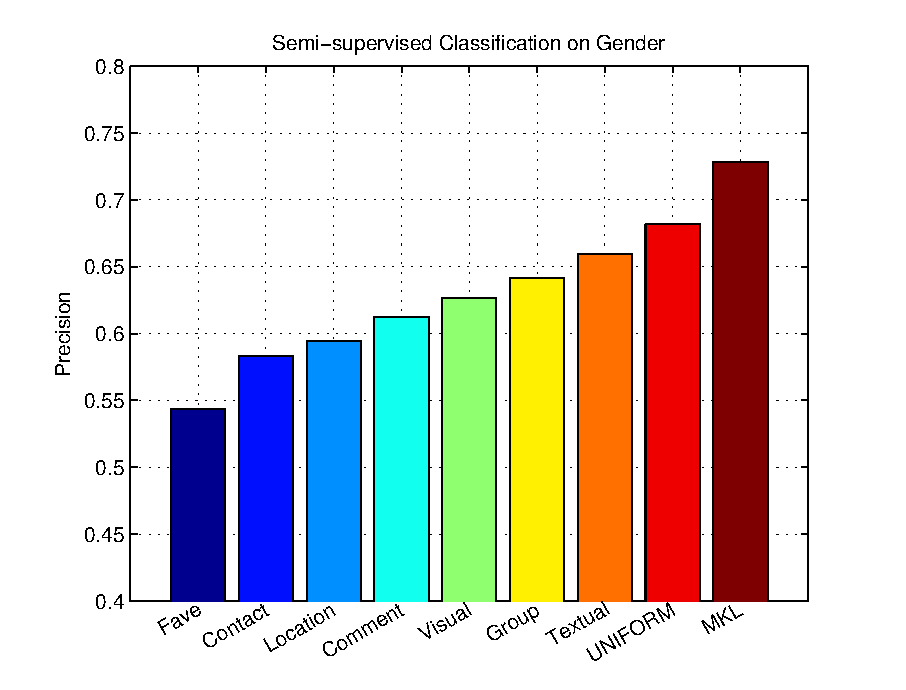
\includegraphics[width=12cm]{figures/gender.eps}
\includegraphics[width=12cm]{figures/location.eps}
\hspace{-5mm}
\caption{The evaluation of inferred social strength graph for semi-supervised classification. The left figure is the accuracy of {\em gender} prediction, the
right figure is the accuracy of {\em location}.}
\end{center}
\vspace{-5mm}
\end{figure*}

For both tasks, KTA-MKLR performs best. It is better than uniform combination. This verifies that the modalities are complementary for the evaluated
classification tasks. Regrading the single kernels, {\em Textual} kernel performs the best, even rivals MKL for the location prediction task. Recall this also
holds for the friend and group recommendation task. We can conclude that the tag-based kernel is most effective for SSM. The most possible reason is the
semantic information carried by tags is most meaningful for characterizing the users. On the other hand, among all the 4 tasks, the {\em Fave} kernel performs
worst. Recall that it is defined by the count of photos users like. It is dominated by the quality of photos, instead of social relationship. So it is not very
useful for SSM.

%================================================
\section{Discussion and Related Work} \label{sec:ssm-discussion}
%================================================

Our work in this chapter is closely related to the following research topics.

%++++++++++++++++++++++++++++++++++
\subsection{Data Mining with Flickr Data}
%++++++++++++++++++++++++++++++++++

There exists rich research on mining Flickr data. In \cite{civr/NegoescuG08}, the author conducted probabilistic latent semantic analysis on the Flickr interest
groups, where each group is abstracted to be a collection of tags annotated to the images belonging to this group. This work is group-oriented and it is unclear
how strong the relationship between users is. Due to the subjective and noisy process in group generating and expanding, Negoescu et. al.
\cite{mm/NegoescuAPVG09}\cite{mm/NegoescuG08} proposed methods to hierarchically organize groups and model users and groups equally. These works are also {\em group-oriented}.

There are works focus on how to make use of the metadata of Flickr images to facilitate other applications. For example, geo-tag analysis
\cite{mm/KennedyNANR07}\cite{sigir/SerdyukovMZ09}, automatic tag annotation\cite{mm/WuHJZY09}, concept / tag modeling\cite{mm/WuHYML08}.These techniques are
related to our work as they analyze both Flickr images and their annotated tags. However, all these studies are {\em image-orientated}, which cannot solve our
{\em user-orientated} problem.

Our discriminative framework predicts the social strength between two arbitrary input users. It incorporates the rich content and context information on Flickr
effectively, whereas previous work cannot make use of multiple modalities effectively.

%++++++++++++++++++++++++++++++++++
\subsection{Social Strength Modeling}
%++++++++++++++++++++++++++++++++++

Our task in this work is to infer the social strength among Flickr users. This connects to social strength modeling or link predictions, where quite a few
representative works exists, e.g., \cite{sn/AdamicA01,nips/TaskarWAK03,www/SinglaR08,chi/GilbertK09,www/XiangNR10,www/LeskovecHK10,www/ChoudhuryMHW10}. However,
few existing works make use of the rich content+context data of Flickr images to infer the social relationship between Flickr users. Moreover, our motivation
here is to help users find out who exhibits similar interest in photo sharing. Thus our technique should be content driven, instead of mutual
communication-based on traditional works.

The unique characteristics of Flickr data provides more flexibility in social network mining. The idea of using Flickr data to infer social relationships has
been recently proposed \cite{mm/WuT09, cvpr/SinglaKLG08, icmcs/YuJL09}. Wu et. al. \cite{mm/WuT09} tried to reveal the closeness of people by face detection
techniques. However, this work is severely limited by the range of useable images. Singla et. al. \cite{cvpr/SinglaKLG08} identified the social relationships
between individuals in consumer photos with the principled Markov logic networks. Due to the diversity of the images in Flickr, this rule based method is not
applicable for our task here. Yu et. al. \cite{icmcs/YuJL09} intended to recommend a user's images to a known interest group based on supervised classification
where the initial group membership is deemed as label information. As we aforementioned, the initial group membership is subjective, incomplete, and noisy,
which may not be reliable enough to serve as supervised information.

Very recently, Xiang et. al. proposed a hybrid generative-discriminative model which assumes a latent variable measuring the social strength computed from the
user profile similarities\cite{www/XiangNR10}. The interactive activities are results of such latent variables. However, the profile data of Flickr is not so
complete since it is not initially designed to be a social network site. It is not sufficient to infer the social strength solely based on the profile
similarities. In addition, separating the interaction graph from profile similarity graph increases modeling complexity.

%++++++++++++++++++++++++++++++++++
\subsection{Multiple Kernel Learning to Rank}
%++++++++++++++++++++++++++++++++++

Our main technique is built on two topics, {\em kernel learning} and {\em learning to rank}. The most crucial element of a kernel method is {\it kernel}, which
is in general a function that defines an inner product between any two examples in some induced Hilbert space~\cite{Cristianini00}. Recent years have witnessed
the active research of learning effective kernels automatically from data~\cite{jmlr/LanckrietCBGJ03}. The most popular example technique for kernel learning
is
{\em Multiple Kernel Learning} (MKL)~\cite{jmlr/LanckrietCBGJ03,jmlr/SonnenburgRSS06,jmlr/RakotomamonjyBCG08}, which aims at learning a linear
(or convex) combination of a set of predefined kernels in order to identify a good target kernel for the applications. Besides the work of improving the
efficiency of MKL, a number of extended MKL techniques have been proposed to improve the regular linear MKL
method~\cite{icml/VarmaB09,nips/CortesMR09,nips/KloftBSLMZ09,icml/CortesMR10}. Here we adopt the two-stage method of Cortes et. al.\cite{icml/CortesMR10} as it
is computationally simple and works well both theoretically and practically. We learn the weight of each modality by maximizing the inner product between the
combined kernel and the target kernel, which can be task dependent to make our solution more flexible.

Learning to rank is an active research topic in machine learning and information retrieval (IR) community (refer to \cite{sigir/Liu10}). It provides a
principled and effective paradigm for IR applications. Here we are aware that the social strength essentially ranks the degree of affinity among people. If we
can rank such relationship properly, we solved the SSM problem. Thus, we borrow the key idea of learning to rank to use and rectify the kernels learned in the first stage.

Instead of detecting binary social ties in traditional social network mining works, we study how to infer the continuous social strength in
multimedia communities. The learned graph is more delicate and informative and can be applied in a lot of important applications, including friend prediction, item recommendation, visualization, etc. Our key idea consists of three components: 1) leverage the multiple data sources to compute multiple similarity functions, which can be enforced to satisfy positive semi-definite property to construct valid kernels; 2) employ the kernel target alignment algorithm to learn the weight of each modality and use the weighted summation of base kernels as the ideal kernel; 3) devise the learning to rank framework based on the learned kernel to infer the social strength. Our techniques are are purely discriminative and do not require any assumption of the underlying parametric statistical models that governs the social strength. Empirical results verifies its efficacy. We open this work can call more attention to SSM on multimedia communities.
